\section{Trajectory Compression}
\label{sec:traj}
\subsection{Methods in Trajectory Compression}
A trajectory is a sequence of geospatial points that represents a path. Optionally, a timestamp of the point registration can also be stored. The goal of compression is to reduce the size of the trajectory by storing in a compressed form. This is measured by the compression ratio, which is the ratio between the uncompressed and compressed data. Trajectory compression can be classified into three main categories: streamed/batched, lossless/lossy, and spatial-only/spatio-temporal.

The primary distinction between streamed and batched compression lies in the amount of data processed at a time. Batched compression is generally simpler because it allows access to the entire trajectory at once. In contrast, streamed compression can only handle one segment at a time due to memory limitations, which prevents loading the entire trajectory. This limitation complicates the process as the complete scope of the trajectory remains unknown. A common approach for managing streamed data is the use of a Sliding Window, which forms the basis of many algorithms. Batched compression, on the other hand, requires more storage and concentrated processing power. It necessitates loading the entire trajectory onto disk and processing it in a single operation. Due to its additional resource requirements and knowledge of the entire trajectory, batched compression outperforms streamed compression in terms of compression ratio and accuracy. Nonetheless, streamed compression can be advantageous in certain situations. Its ability to compress data as it is received, eliminating the need for intermediate storage, can outweigh the superior compression achieved by batched methods in terms of practicality. In addition it's absolutely necessary for real time systems.% Build on real time systems

Lossy algorithms sacrifice accuracy for more efficient storage. Lossless algorithms reduce the size without losing any information. They generally have worse performance than lossy algorithms as a result of this. Within lossy compression, there is a trade-off of "how lossy." This means that you can balance the fidelity of the compression with the compression ratio. Greater fidelity results in lower compression ratio, and vice versa. This is called "bounded lossy compression". Modern algorithms, such as REST, perform bounded lossy compression, rather than a binary choice between lossy or lossless compression.

The distinction between spatial-only and spatio-temporal lies in the consideration of the temporal aspect, that is, whether time is taken into account or not. Spatial-only compression focuses solely on the spatial differences between trajectories. \cite{SpatiotemporalComp}, define two spatiotemporal concepts that can improve trajectory compression: \textit{time-ratio distance} and \textit{speed difference threshold}.

The time-ratio distance represents the distance between two synchronized points: one point from the original trajectory and another point from the compressed trajectory. The traditional error metric used in compression is the perpendicular distance between a point and the new trajectory. However when using synchronized points the distance will change based on time. This was first defined by \cite{SpatiotemporalComp} and has now been formalized under the term Synchronized Euclidean Distance (SED). Figure \ref{fig:sed} illustrates the concept of time-ratio distance, which will be further discussed in section \ref{subsub:SED}

The speed difference threshold is the concept of comparing speeds between sequential segments of the trajectory. The speed is not expected to be directly in the data; rather it iss calculated as $ \Delta d / \Delta t $, where \textit{d} is distance and \textit{t} is time. When the speed difference is large this indicates a sudden movement or turn. These points are considered important for the internal shape of the trajectory. Therefore, ensuring no points with a speed difference larger than a certain threshold are removed during compression can increase the fidelity of the trajectory when considering the temporal aspect.

The results in the experiments by \cite{SpatiotemporalComp} show that implementing time-ratio distance and a speed difference threshold had a slight improvement in compression ratio and a significant reduction of error. Although the error metric was spatiotemporal and the algorithms used in comparison were not, therefore the results are not that surprising. Meanwhile, \cite{Sun2016} claims that spatiotemporal is simple and efficient with the ability to maintain internal features in trajectories. However, they are unpopular because existing algorithms only consider speed which may lead to greater errors and break the holistic geometrical characteristics of trajectories.


\subsection{Accuracy Metrics}
The fidelity of a compression can be measured by different accuracy metrics. This is done by calculating the distance between each point in the original trajectory and the new trajectory. From these distances, various operations can be performed to obtain an overall metric. The mean distance of all points is the most commonly used measure, but other metrics such as median or maximum can also provide valuable insights into accuracy. The method used to calculate the distance, determines the accuracy metric. Example distances are shown in figure \ref{fig:sed}. The following sections will explore the most used accuracy metrics, as menioned by, \cite{TrajFramework} and \cite{Sun2016}.

\subsubsection{Perpendicular Distance}
\label{foobar:PD}
Perpendicular distance (PD) refers to the shortest distance from a removed point to the new trajectory, as shown in figure \ref{fig:sed}. The shortest distance is always perpendicular to the trajectory, hence the name.

\subsubsection{Synchronized Euclidean Distance}
\label{subsub:SED}
SED is a measurement where a point $p_{i}$ is assigned a distance to the new trajectory that is equal to the distance to the synchronized point $p'_{i}$, as shown in figure \ref{fig:sed} $p'_{i}$ is calcluated as:
\begin{equation}
    \begin{aligned}
        t'_{i} & = t_{i}                                                \\
        x'_{i} & = x_{s} + \frac{t_{i}-t_{s}}{t_{e}-t_{s}}(x_{e}-x_{s}) \\
        y'_{i} & = y_{s} + \frac{t_{i}-t_{s}}{t_{e}-t_{s}}(y_{e}-y_{s}) \\
    \end{aligned}
\end{equation}
This error metric takes time into account. Two trajectories traversing the exact same spatial points might still be considered different if one took a longer time. This can be a useful metric for differentiating between taxi trips in rush hour and outside rush hour, since the trips outside rush hour will typically be shorter in duration.

\begin{figure}[ht]
    \begin{minipage}[b]{0.5\linewidth}
        \centering
        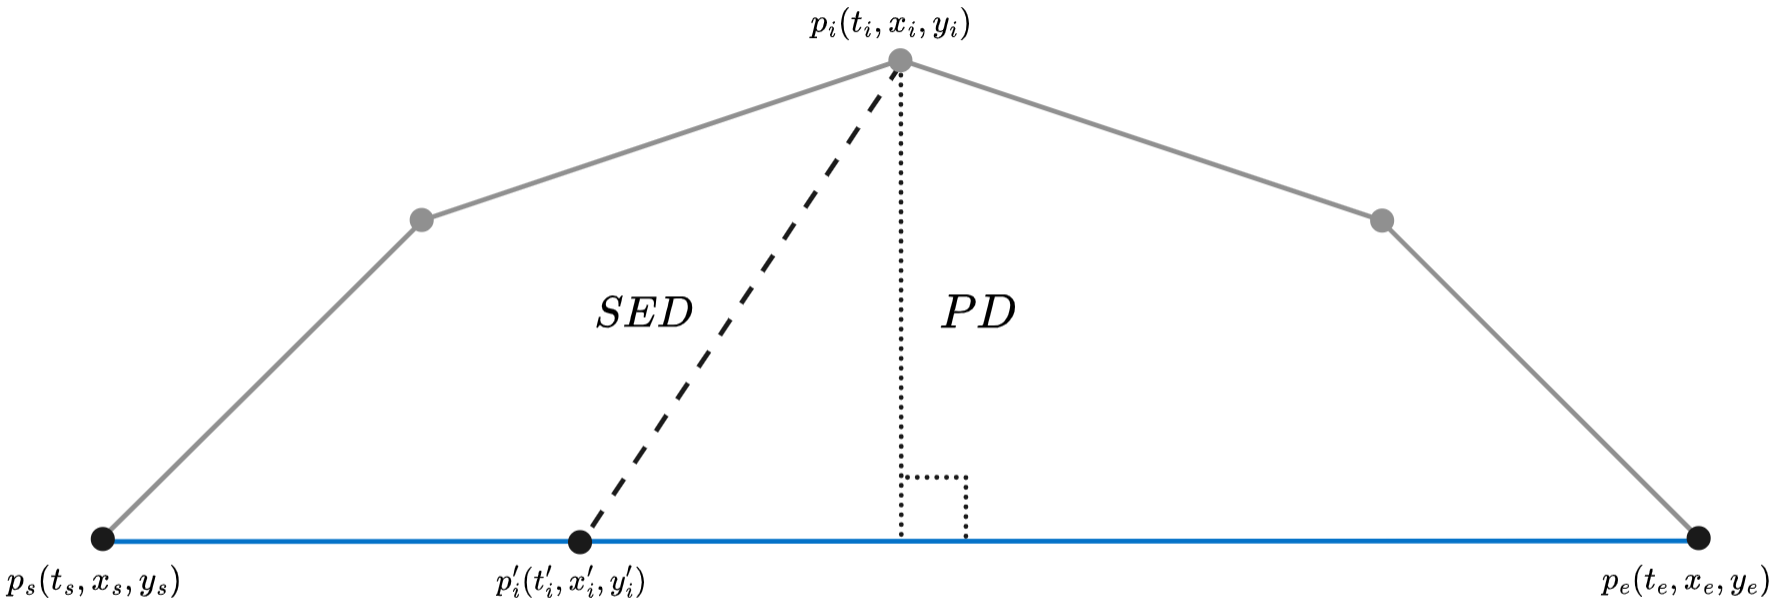
\includegraphics[width=\linewidth, height=7cm, keepaspectratio]{./figures/sed.png}
        \caption{Original trajectory in gray and new trajectory in blue showing distances SED and PD.}
        \label{fig:sed}
    \end{minipage}
    \begin{minipage}[b]{0.5\linewidth}
        \centering
        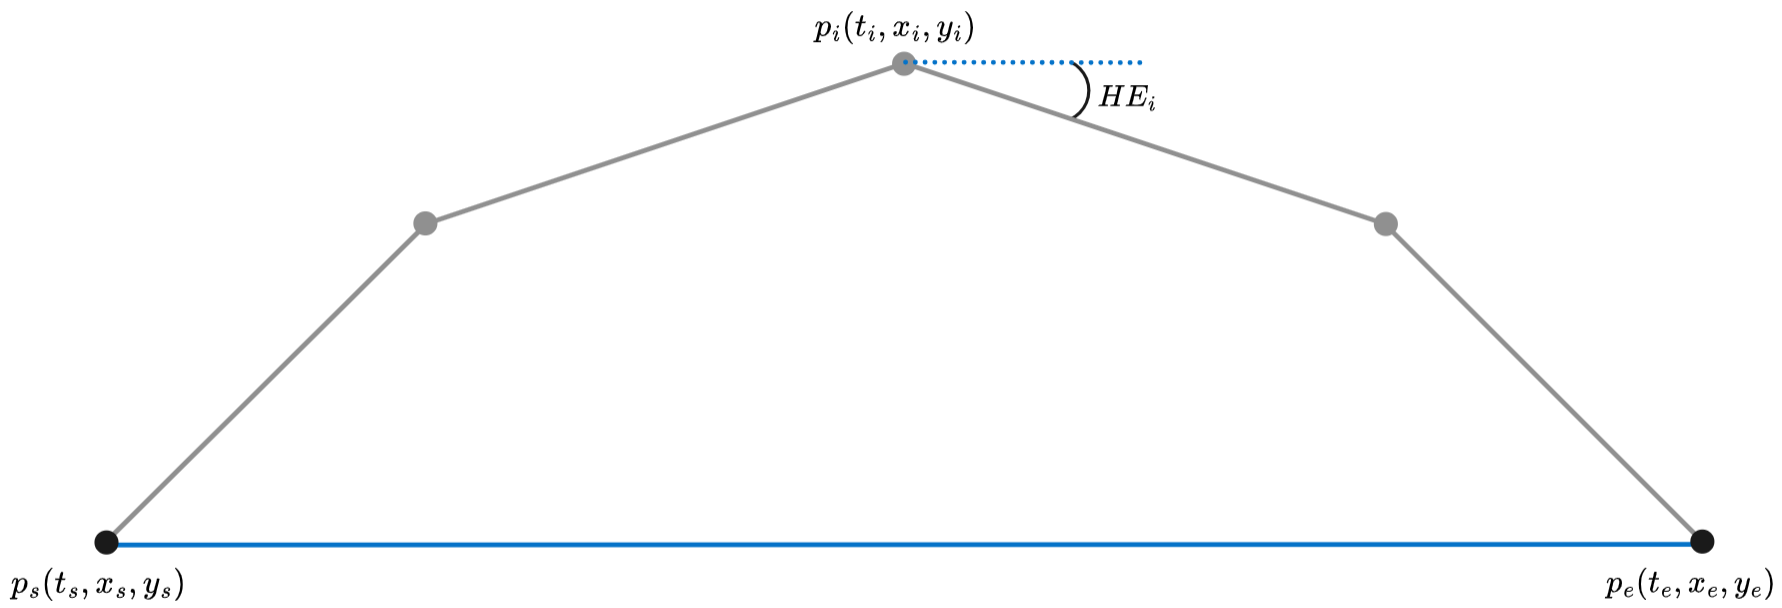
\includegraphics[width=\linewidth, height=7cm, keepaspectratio]{./figures/heading_error.png}
        \caption{Original trajectory in gray and new trajectory in blue showing distances HE.}
        \label{fig:hed}
    \end{minipage}
\end{figure}

\subsubsection{Heading Error}
The Heading Error (HE) for a point $p_{i}$ is the angular difference between the line segment $p_{i}$-$p_{i+1}$ along the original trajectory and $p'_{i}$-$p'_{i+1}$ along the compressed trajectory shown in figure \ref{fig:hed}. The angle represents the difference in direction between the original and the compressed trajectory at a given point. This metric is useful for detecting erratic movement and disruption of traffic flow according to \cite{TrajFramework}.

\subsubsection{Speed Error}
The Speed Error is similar to the Heading Error in that it compares the segments from the original trajectory with the corresponding segment in the compressed trajectory. However, it compares speed instead of direction. The Speed Error is the difference in speed between the original and compressed trajectory at a given point.

\subsubsection{Dynamic Time Warping}
Dynamic Time Warping (DTW) is an algorithm used to determine the alignment cost between two time series. It can align the series by finding which points correspond to each other and the distortion between corresponding points. The total alignment cost describes how similar the series are according to the DTW measure. When trying to align two very different series, the alignment cost will be high, for two similar series, it will be low. With regards to trajectory compression, the alignment cost between a compressed trajectory and the original describes how similar they are, or how much information is preserved in compressed form. A compression with high fidelity will have a low alignment cost.

The DTW algorithm works by calculating the distance matrix between two series. The distance $d_{i,j}$ in a matrix $D$ between the series $A$ and $B$ is given by:
\begin{equation}
    \label{eq:dtw}
    \begin{aligned}
        d_{i, j} & = distance(A_{i}, B_{j}) + \min \left\{ \begin{aligned}
                                                                & d_{i-1, j-1} \\
                                                                & d_{i-1, j}   \\
                                                                & d_{i, j-1}
                                                           \end{aligned} \right\}
    \end{aligned}
\end{equation}
From equation \ref{eq:dtw} we see that the distance $d_{i, j}$ is dependent on the previously calclulated distances, for the first point $A_{1}$ and $B_{1}$ the previous points wont be defined. Therefore the DTW algorithm initializes $d_{0,0} = 0$, $d_{0, 1}...d_{0, n} = \infty$ and $d_{1, 0}...d_{n, 0} = \infty$. The initialization values can be seen in table \ref{dtw_distance}. The algorithm also needs a distance function, for example PD or SED, the choice depends on the type of data and the purpose of the DTW measure. Afterwards the values are calculated one by one from the top row to the bottom. In table \ref*{dtw_distance} the previous points that are used to calclulate $d_{2,2}$ is highlighted in red. As we can see the minimum of the red values is $d_{1,1} = 1$ which gives $d_{2, 2} = distance(A_{2}, B_{2}) + 1$. The alignment cost is the final distance calculated, $d_{5,5}$ in figure \ref*{dtw_distance}, or more generally $d_{n,n}$.

\begin{table}[h]
    \centering
    \begin{tabular}{|c|c|c|c|c|c|c|}
        \hline
        \multicolumn{1}{|c|}{\diagbox{$A_{i}$}{$B_{j}$}} & 0        & 1                    & 2                    & 3        & 4        & 5         \\ \hline
        0                                                & 0        & $\infty$             & $\infty$             & $\infty$ & $\infty$ & $\infty$  \\ \hline
        1                                                & $\infty$ & $\textcolor{red}{1}$ & $\textcolor{red}{3}$ & $1$      & $0$      & $4$       \\ \hline
        2                                                & $\infty$ & $\textcolor{red}{3}$ & $d_{2,2}$            & $$       & $$       &           \\ \hline
        3                                                & $\infty$ & $$                   & $$                   & $$       &          &           \\ \hline
        4                                                & $\infty$ & $$                   & $$                   &          &          &           \\ \hline
        5                                                & $\infty$ & $$                   &                      &          &          & $d_{5,5}$ \\ \hline
    \end{tabular}
    \caption{The DTW Distance Matrix between $A$ and $B$ halfway finished. The next point to calculate is $d_{2,2}$.}
    \label{dtw_distance}
\end{table}

\subsubsection{Max Dynamic Time Warping}
This is a variant of Dynamic Time Warping which changes the distance equation by taking the max of the distance and the former minimum instead of taking the sum. The new equation is \begin{equation}
    \label{eq:max_dtw}
    \begin{aligned}
        d_{i, j} & = max(distance(A_{i}, B_{j}), \min \left\{ \begin{aligned}
                                                                   & d_{i-1, j-1} \\
                                                                   & d_{i-1, j}   \\
                                                                   & d_{i, j-1}
                                                              \end{aligned} \right\})
    \end{aligned}
\end{equation}
Following the previous example, $d_{2, 2} = max(distance(A_{2}, B_{2}), 1)$




\subsection{Performance Metrics}
\subsubsection{Compression Ratio}
Compression ratio measures the amount of data compressed. This is calculated as $C_{r} = \frac{|o|}{|c|}$, where $C_{r}$ is the compression ratio, $|o|$ is the size of the original data, and $|c|$ is the size of the compressed data. Storing a 10GB file with 5GB gives a compression ratio of $10 / 5 = 2$, meaning it was stored using half the original size. This can also be written as a 2:1 compression ratio.

\subsubsection{Compression Performance}
Compression performance measures the speed of compression as well as the resource usage. Compression speed is simply the time it took to compress measured in seconds. Resource usage, however can be measured in a variety of ways, this depends on what kind of usage you want to measure, for example memory usage or CPU time. Computer executions like these have variance in performance, therefore it is important to measure the average for multiple runs when doing an experiment, both for compression speed and resource usage. Additionally it is important that when comparing compression performance that the measures were gathered in the same environment, meaning the experiment was executed on the same computer with the same version of the program. Otherwise the results are not comparable.